\documentclass{article}
\usepackage{microtype}
\usepackage{times}
\usepackage{helvet}
\usepackage{courier}
\usepackage{pdfpages}
\usepackage{graphicx}
\usepackage{algorithm}
%\usepackage[ruled,vlined]{algorithm2e}
\usepackage{algorithmic}
\usepackage{float}
\usepackage{caption}
\usepackage{subcaption}
\usepackage{url}
\usepackage{amsmath, amssymb, mathrsfs}
\frenchspacing
\setlength{\pdfpagewidth}{8.5in}
\usepackage{setspace}

\usepackage{hyperref}

\usepackage{icml2019}
%\usepackage[accepted]{icml2019}

\newtheorem{theorem}{Theorem}
\newtheorem{definition}{Definition}
\newtheorem{lemma}{Lemma}
\newtheorem{proof}{Proof}

%\SetKwInOut{Initialization}{Initialization}


\setlength{\pdfpageheight}{11in}
%\pdfinfo{
%/Title (Insert Your Title Here)
%/Author (Put All Your Authors Here, Separated by Commas)}
%\setcounter{secnumdepth}{0}
\begin{document}
% The file aaai.sty is the style file for AAAI Press
% proceedings, working notes, and technical reports.
%
\twocolumn[
\icmltitle{Compiler-Level Matrix Multiplication Optimization for Deep Learning}

% It is OKAY to include author information, even for blind
% submissions: the style file will automatically remove it for you
% unless you've provided the [accepted] option to the icml2019
% package.

% List of affiliations: The first argument should be a (short)
% identifier you will use later to specify author affiliations
% Academic affiliations should list Department, University, City, Region, Country
% Industry affiliations should list Company, City, Region, Country

% You can specify symbols, otherwise they are numbered in order.
% Ideally, you should not use this facility. Affiliations will be numbered
% in order of appearance and this is the preferred way.


\begin{icmlauthorlist}
\icmlauthor{Huaqing Zhang}{petuum}
\icmlauthor{Xiaolin Cheng}{huawei}
\icmlauthor{Hui Zang}{huawei}
\icmlauthor{Dae Hoon Park}{huawei}
\end{icmlauthorlist}

\icmlaffiliation{petuum}{Petuum, Inc, Sunnyvale, CA, USA}
\icmlaffiliation{huawei}{Huawei Research, Santa Clara, CA, USA}

\icmlcorrespondingauthor{Huaqing Zhang}{huaqing.zhang@petuum.com}
\icmlcorrespondingauthor{Hui Zang}{hui.zang@huawei.com}

% You may provide any keywords that you
% find helpful for describing your paper; these are used to populate
% the "keywords" metadata in the PDF but will not be shown in the document
\icmlkeywords{Machine Learning, ICML}

\vskip 0.3in
]

\printAffiliationsAndNotice{\icmlEqualContribution}
%\author{Huaqing Zhang, Xiaolin Cheng, Hui Zang, Dae Hoon Park\\
%Huawei Research, USA.\\
%}
%\maketitle

\begin{abstract}
As an important linear algebra routine, GEneral Matrix Multiplication (GEMM) is considered a fundamental operator in deep learning. Compilers need to translate these routines into low-level code optimized for specific hardware. Compiler-level optimization of GEMM has significant performance impact on training and executing deep learning models. However, current deep learning frameworks rely on hardware-specific operator libraries in which GEMM optimization has been mostly achieved by manual tuning, restricting the performance of deep learning frameworks on different target hardware. In this paper, we propose two novel algorithms for GEMM optimization based on the TVM framework. The Greedy Best First Search (G-BFS) guided method is a lightweight method based on search. The Neighborhood Actor Advantage Critic (N-A2C) method is based on reinforcement learning. Experimental results show significant performance improvement of both approaches over state-of-the-art optimization methods, in terms of computation time and the fraction of space explored. The proposed approaches have potential to be applied for other operator-level optimization.
\end{abstract}


\section{Introduction}
In recent years, deep learning has been attracting increasing attention from both academia and industry~\cite{lecun2015deep}. With its own advances in algorithmic and architectural design, significant improvement in computational hardware (e.g. GPU and TPU), and availability of enormous amount of labeled data, deep learning has shown success in many domains, such as computer vision, natural language processing, speech recognition, health care, finance, etc. There is no doubt that deep learning solutions will be adopted in even more areas in the upcoming years. 
%It shows promising potential with superior performance and broader penetration in every aspect of IT technology. 
% Inspired by biological nervous systems, deep learning takes advantage of the large computation power nowadays by applying computational models of multiple processing layers to learn representations of data with multiple levels of abstraction \cite{lecun2015deep}. The approach achieves significant performance improvement in the areas of computer vision, natural language processing, audio, biology and game industry, and show promising potentials with higher performance and boarder applications in future. 


% However, with the increasing development in machine learning and deep learning, it becomes difficult for non-machine learning experts to efficiently apply deep learning models to solve real-world problems. In order to make deep learning much easier to be applied and achieve good performance, automated Machine Learning (AutoML) has attracted remarkable attentions, which can autonomously apply suitable machine learning and deep learning models to analyze the potentials of the data and provide beneficially suggestions. Lots of AutoML services and libraries, including AutoWEKA, Auto-sklearn, TPOT, H2O AutoML, Google CLOUD AUTOML, have been developed nowadays and helps both developers and researchers in the areas of artificial intelligence. 

%%%%%%%%%%%%
% https://www.ml4aad.org/automl/
%AutoML systems

However, computing deep learning models (both training and inference) efficiently on various hardware is a difficult task, which involves end-to-end compiler optimization at several levels from computational graphs to operators, and down to executable code on target hardware~\cite{Chen18}. A computational graph is a global view of operators and data flow among them. Within a graph, operators specify various computation that is required for individual operations on tensors. Current optimization techniques at the computational graph level are hardware agnostic and independent from the implementation of operators within a graph. For example, a standard procedure, operator fusion, combines multiple operators into a single kernel, avoiding latency introduced by write-back and loading of intermediate results into memory. At the operator level, existing optimization is mostly limited to specific implementation for a framework (e.g. TensorFlow XLA) or proprietary library for a particular target device (e.g. Nvidia cuDNN). Such libraries have been built mostly based on expert knowledge and manual tuning to perform efficiently and effectively. 

Deep learning models are expected to run on diverse hardware platforms (CPU, GPU, FPGA, ASIC, SoC, etc.) with very different characteristics that can be leveraged to optimize various deep learning operations. To efficiently map deep learning operation/workload to broader range of hardware, TVM has been proposed~\cite{Chen18} as a general compiler framework for automated tensor operator optimization. In this framework, a configuration space can be defined for each operator. Optimization of an operator is to find a configuration that can optimize a performance metric (e.g., the lowest running time). Configuration is the detailed specification of how an operator is computed and executed on target hardware. For example, in matrix multiplication, tiling is required to make computation more efficient, but various tiling strategies may generate configurations that have significantly different performance. Configuration space for individual operators may have different structures and properties. %Current tuning approaches for tensor operators in TVM do not fully exploit useful information that exists among proximal configurations. 

In this paper, we aim at more efficient operator optimization. %further improving the efficiency of configuration tuning. 
We focus on the GEneral Matrix Multiplication (GEMM) operator which is the fundamental operator in deep learning. GEMM computes the product (multiplication) of two matrices and the operator can be translated into nested loops controlled by a fixed set of few parameters. Its optimization can be reduced to finding the optimal combination of parameter values in this set. We analyze structure of its configuration space and design improved tuning approaches for GEMM optimization. The contributions of the paper are three-fold:
\begin{itemize}
\item We consider the relation between different configurations and define the neighboring relation between two configurations. We employ a Markov Decision Process (MDP) for exploration over the configuration space.   
\item Based on the neighboring relations within the configuration space, we propose a Greedy Best-First-Search (G-BFS) guided method and a Neighborhood Actor Advantage Critic (N-A2C) method to search for an optimal configuration given two matrices to be multiplied. %This  for automated compiler-level configuration optimization.
\item We evaluate the performance of our proposed methods in TVM framework for Nvidia Titan XP GPU. We compared them with state-of-the-art GEMM tuners using XGboost~\cite{chen2016xgboost} and RNN controller~\cite{Chen18}. We demonstrate that both our methods can discover high-performance configurations efficiently with smaller fraction of explored configuration space and shorter time to complete. By exploring only 0.1\% of the configuration space, our methods discover configurations of {\bf 24\%} less computing cost than what the XGBoost method can find and configurations of {\bf 40\%} less computing cost than what the RNN method can find, for multiplying two $1024 \times 1024$ matrices. 
\end{itemize}
\subsection{Related Work}

As there are multiple AI frameworks and a wide range of hardware involved in deep learning applications nowadays, it is important but challenging for compiler-level optimization to efficiently and flexibly harmonize AI algorithms with the underlying hardware and optimize the performance of various deep learning applications. Much work has explored this space and achieve good performance improvement. CuDNN \cite{chetlur2014cudnn} provides highly efficient implementations of various deep neural network layers and it is considered the standard for accelerating deep learning on Nvidia GPUs. NNPACK \cite{dukhan2016nnpack} and PCL-DNN \cite{das2016distributed} similarly provide accelerations in x86 processors. Latte \cite{truong2016latte} provides a natural abstraction for specifying new layers and applies domain-specific and general computation graph optimization. XLA (Accelerated Linear Algebra) \cite{leary2017xla} optimizes TensorFlow computations in terms of speed, memory usage, and portability via just-in-time (JIT) compilation or ahead-of-time (AOT) compilation.

However, the aforementioned approaches perform either graph-level or operator-level optimization during compilation and they are not generic enough to accommodate all AI frameworks and hardware. Based on the structure of Halide \cite{ragan2013halide}, \cite{Chen18} proposes a general end-to-end compilation optimization framework combining Neural Network Virtual Machine (NNVM) \cite{nnvm2017} for computation graphs and Tensor Virtual Machine (TVM) \cite{Chen18} for tensor operators. 
%For tensor operators, e.g., GEMM, the configuration tuning efficiency affects the performance for general deep learning. 
Currently in TVM, a tuning method based on XGBoost \cite{chen2016xgboost} is considered the state-of-the-art method for GEMM configuration optimization and has shown superior performance over other methods \cite{Chen18}. %while great potential still exists based on the current development configuration optimization techniques.

For configuration optimization, the intuitive method is grid search, where all possible configuration candidates are tested sequentially so as to find the configuration with best performance. It guarantees to find the global optimal configurations, but the number of tested configuration candidates grows exponentially with the dimensions of configuration space \cite{bellman2015adaptive}, so its usage is limited in problems with small search space or in combination with manual search \cite{hinton2012practical,lecun2012efficient,larochelle2007empirical}. Random search is proposed where the configurations are randomly selected to be tested, and is shown empirically and theoretically to be more efficient than grid search for configuration tuning \cite{bergstra2012random}.
%has  shown that random search is 

As an instance of Bayesian optimization, sequential model-based optimization (SMBO) shows its strength in configuration tuning by iteratively updating the underlying expected improvement, exploring new data through an acquisition function, and training a regression model \cite{hutter2011sequential,bergstra2011algorithms,hoffman2014modular}. The general method has been widely adopted and implemented  \cite{kandasamy2018neural,snoek2012practical}.

%, and a large number of configuration optimization software libraries including Hyperopt \cite{bergstra2013hyperopt}, Spearmint \cite{snoek2012practical}, GPyOpt \cite{gpyopt2016}, MOE \cite{clark2014moe}, RoBO \cite{klein-bayesopt17} and SMAC3 \cite{smac-2017} are widely implemented in academic and industrial areas.

From another perspective, a series of evolutionary approaches have been explored, including the broad class of genetic algorithms (GA) \cite{Holland1975,Goldberg1989}, differential evolution \cite{Storn1997}, estimation of distribution algorithms \cite{larranaga2001estimation,bosman2007adapted} and particle swarm optimization \cite{kennedy2001swarm}.  Evolutionary strategies (ES) \cite{rechenberg1994evolutionsstrategie,schwefel1977numerische} have shown to perform efficiently in configuration tuning. Based on the concept, Covariance Matrix Adaptation Evolution Strategy (CMA-ES), first proposed by \cite{hansen2001completely}, has shown excellent performance by smartly update the mean, step size and covariance matrix for each evolution \cite{LoshchilovH16} . Natural Evolution Strategies \cite{wierstra2014natural} applies natural gradients to update configuration search policy so as to achieve high expected fitness and discover the high-performance configuration.

% In general EA, for every searching iterations of EA, a population of configurations are firstly generated through mutation. After evaluating the fitness of the candidates, the highest scoring configuration candidates are preserved and recombined to form the new population for the next generation. The iteration continues until the optimal configuration candidates are discovered and converged \cite{salimans2017evolution}.

Recently, researchers at Google apply deep reinforcement learning with a RNN controller to optimize the configurations of neural network architectures and its components \cite{bello2017neural,mirhoseini2017device,ramachandran2018searching,zoph2016neural,pham2018efficient}. The excellent tuning performance in wide range of applications shows the potential of deep reinforcement learning in the configuration tuning area. 




\section{Problem Statement}
\subsection{Matrix Multiplication}
Matrix multiplication is a critical operation in many machine learning algorithms, particularly in the domain of deep learning. Training parameters (weights) of a deep neural network in a vectorized fashion essentially involves multiplication of matrices with various sizes. 

Fully-Connected (FC) layers (Fig.~\ref{fig:fc}) and convolutional (Conv) layers (Fig.~\ref{fig:cnn}) are building blocks of feed-forward and convolutional neural networks~\cite{Warden15}. It is straightforward to identify matrix multiplication in computing output value of a FC layer: each input has $k$ elements, and FC layer has $n$ neurons each with $k$ weights. An FC layer is the multiplication of a $m \times k$ matrix ($m$ is sample size) and a $k\times n$ matrix. A Conv layer appears to be a specialized operation, but it can be computed with matrix multiplication after rearranging data in a matrix format: each depth-wise (channel) slice of input can be added into an input matrix as a row; similarly each kernel can be added into a kernel matrix as a column. Convolution operation becomes multiplication of those two matrices. When using AlexNet on image classification with ImageNet dataset, vast majority of computation time on forward pass (94.7\% on GPU, and 88.7\% on CPU) is consumed by Conv and FC layers~\cite{Jia14}.

\begin{figure}[t]
    \centering
    \begin{subfigure}[b]{0.2\textwidth}
    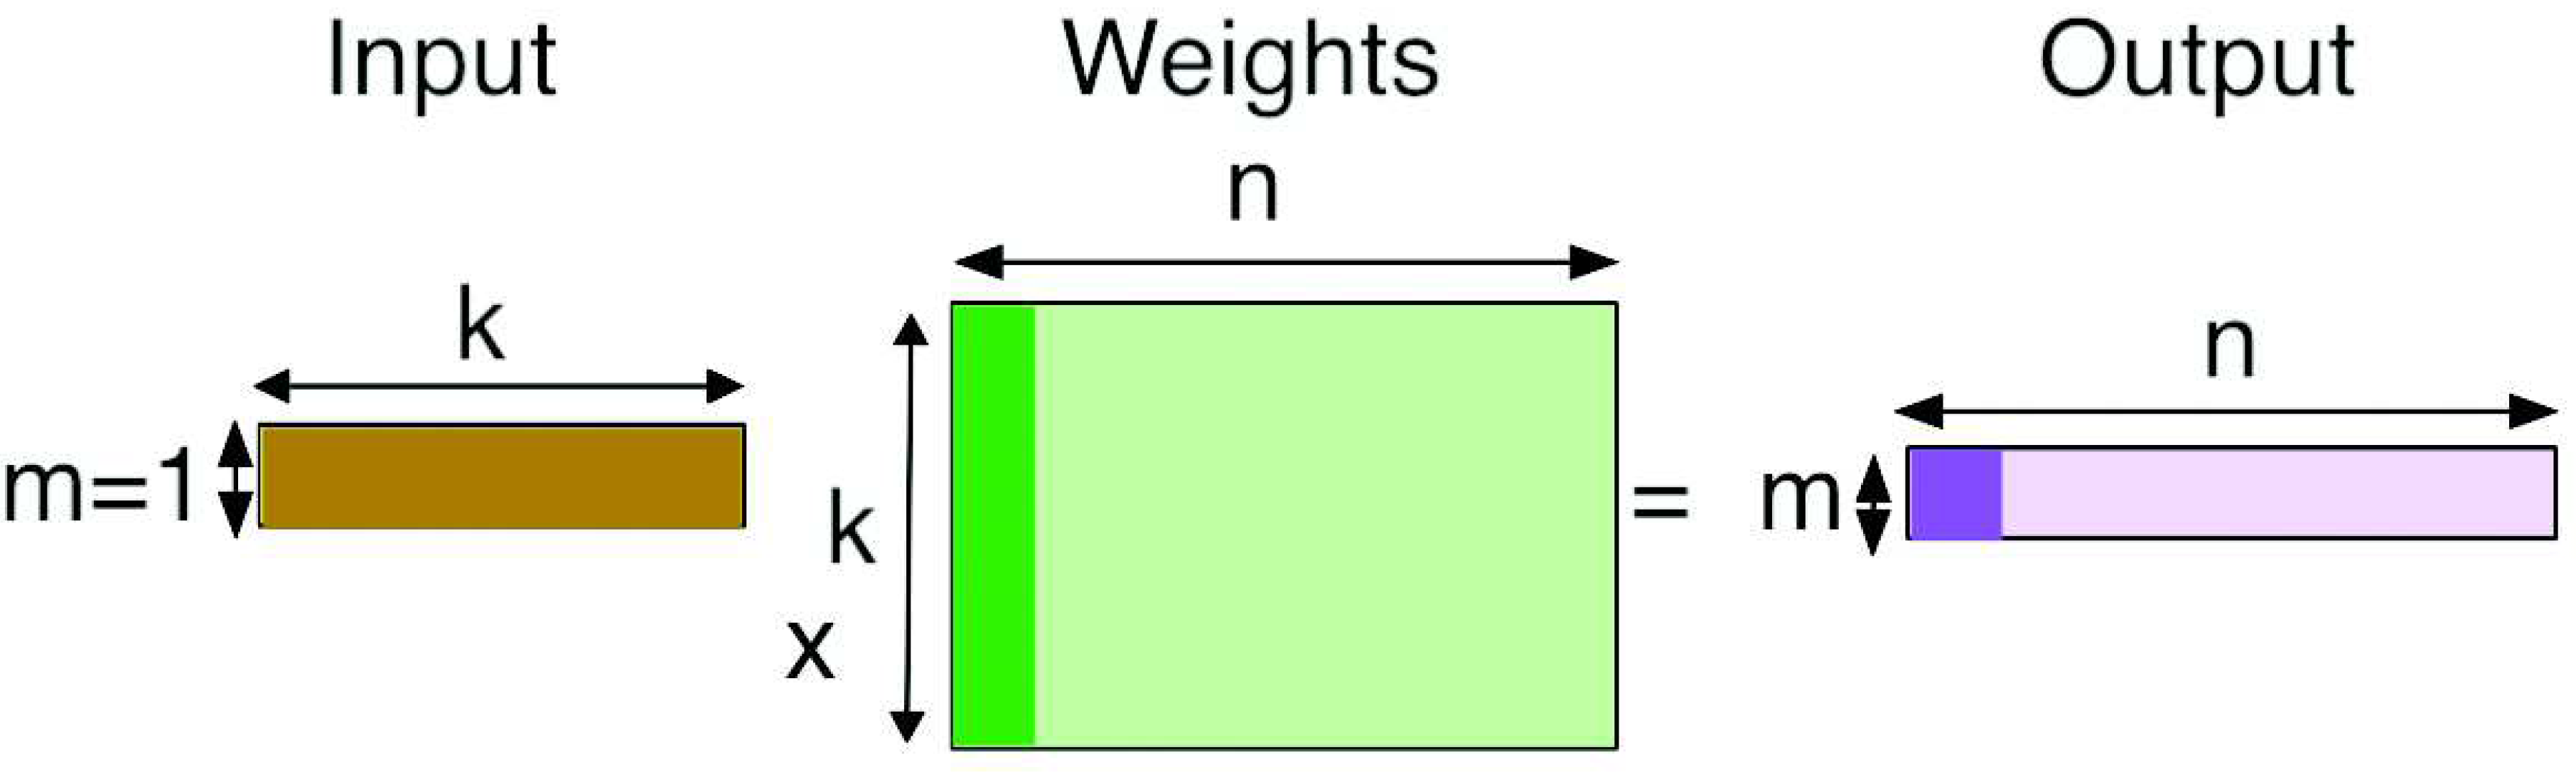
\includegraphics[width=\linewidth]{3_GEMM_backgrounds/fc.png}
    \caption{Fully-Connected Layer}
    \label{fig:fc}
    \end{subfigure}
    \hspace{0.2in}
    \begin{subfigure}[b]{0.2\textwidth}
    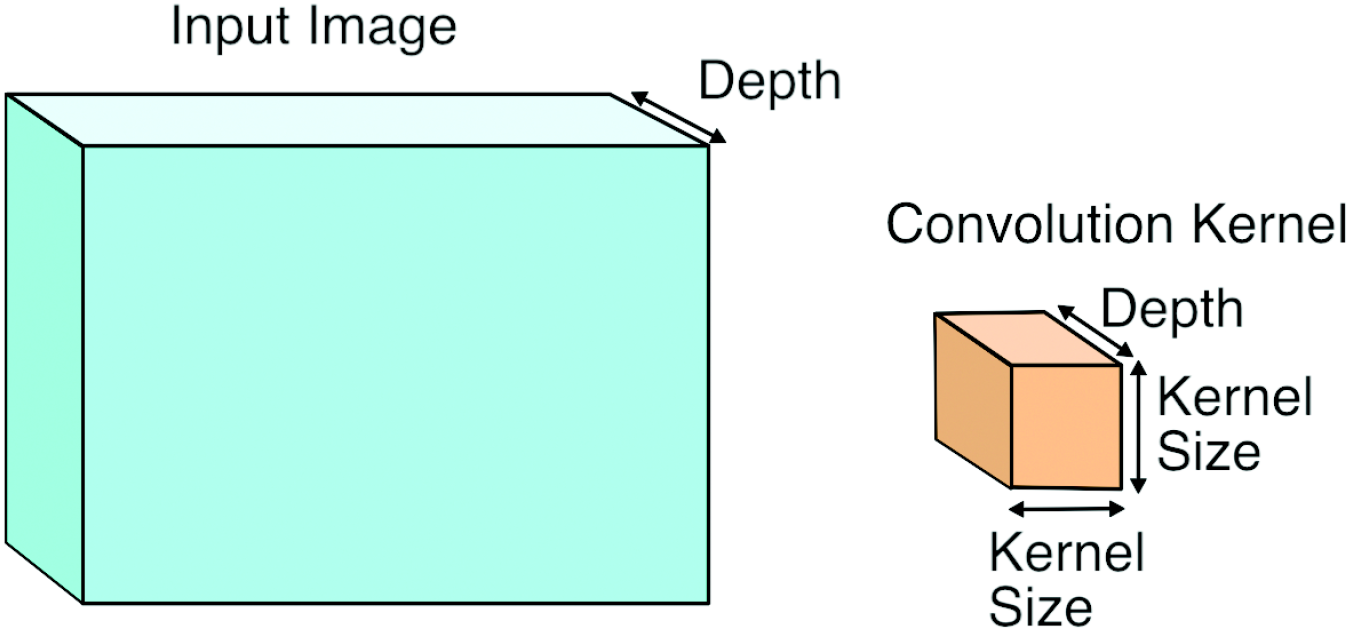
\includegraphics[width=\linewidth]{3_GEMM_backgrounds/cnn.png}
    \caption{Convolutional Layer}
    \label{fig:cnn}
    \end{subfigure}
    \caption{Illustration of deep neural network layers}
    \label{fig:layers}
\end{figure}


% \begin{figure}[h]
%     \vspace{-0.5in}
%     \centering
%     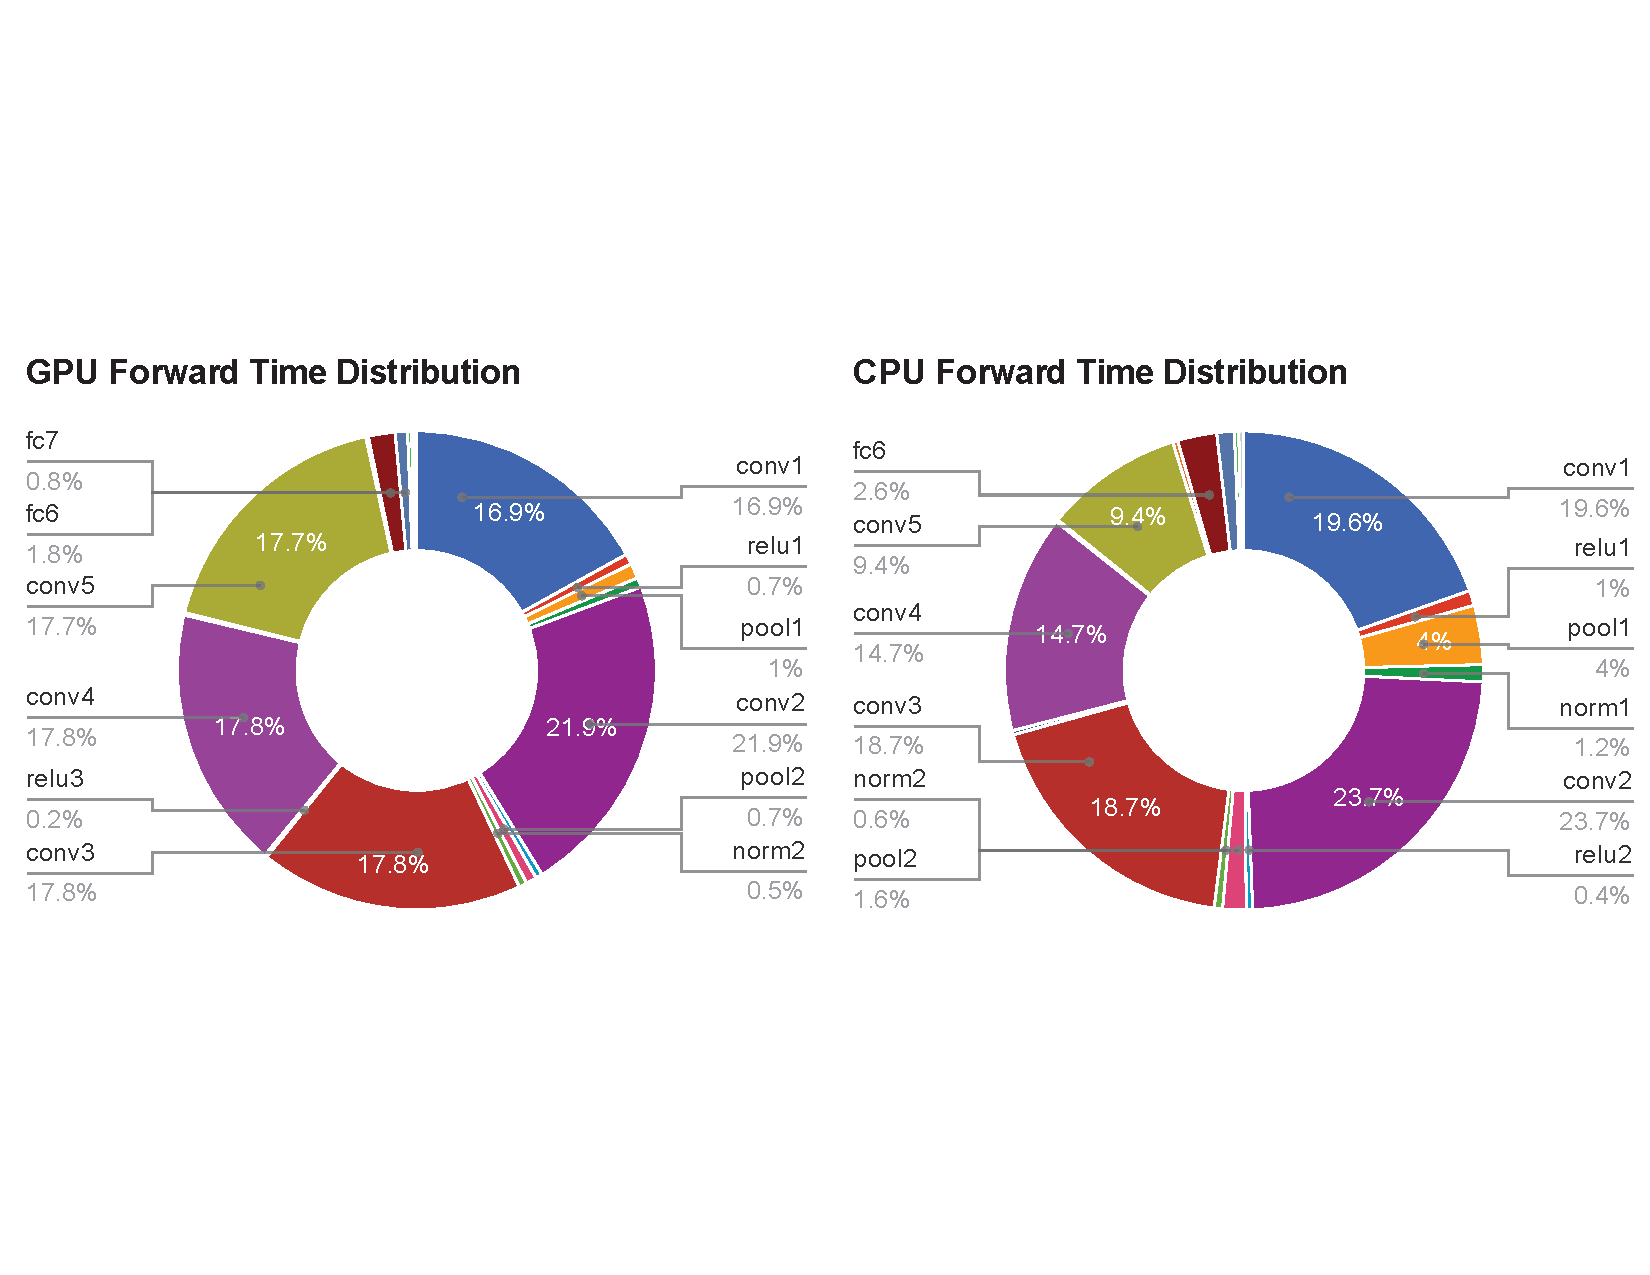
\includegraphics[width=3.2in]{3_GEMM_backgrounds/cnn_time_distribution.pdf}
%     \vspace{-0.5in}
%     \caption{Breakdown of CNN computation time}
%     \label{fig:cnn_time}
% \end{figure}

\subsection{GEMM and Matrix Tiling}
%GEneral Matrix Multiplication (GEMM) is initially part of the BLAS (Basic Linear Algebra Subprograms) library \cite{BLAS2002}. It has the following iterative form:
%\begin{equation}
%    C \Leftarrow \alpha AB + \beta C \nonumber.
%\end{equation}

GEMM is a general procedure ubiquitously used in linear algebra, machine learning, statistics, and many other areas and is implemented in the BLAS (Basic Linear Algebra Subprograms) library \cite{BLAS2002}. It multiplies two input matrices to produce an output matrix. The key difference between GEMM in deep learning and regular matrix multiplication is that the input matrices handled in deep learning are normally much larger. For example, a single layer in a typical convolution neural network may require multiplication of a $256 \times 1024$ matrix by a $1024\times 128$ matrix to produce a $256 \times 128$ matrix. Regular three-for-loop (Fig.~\ref{fig:three}) computation requires 34 million ($256 \times 1024 \times 128$) floating point operations (FLOPs). Modern deep neural networks may have hundreds of convolutional layers (e.g. ResNet152~\cite{He15}), and such networks may need several billions of FLOPs to finish operations in all layers for an input image. 

\begin{figure}[h]
    \centering
    \vspace{-0.1in}
    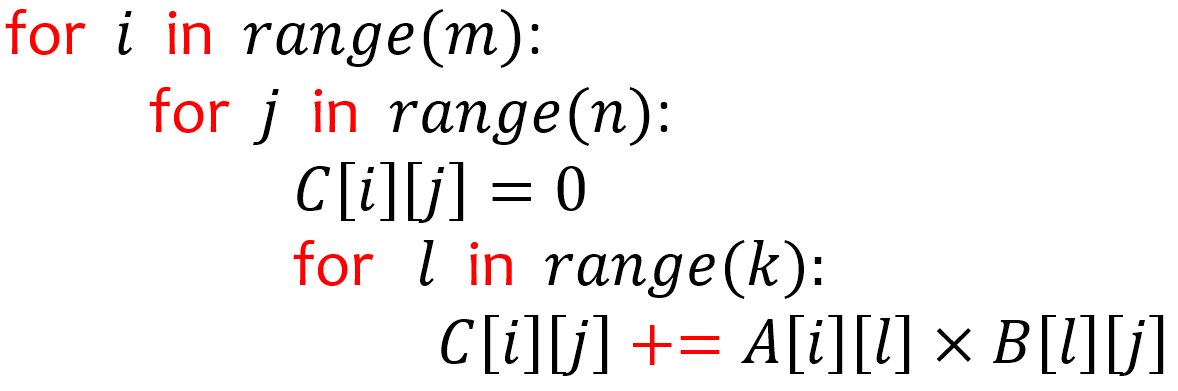
\includegraphics[width=2in]{3_GEMM_backgrounds/three_for_loop.png}
    \vspace{-0.1in}
    \caption{Computing matrix multiplication}
    \label{fig:three}
\end{figure}

High cache hit rate of memory access is critical for complex numerical computation, such as GEMM. The large sizes of matrices usually forbid the entire matrices being loaded into memory or cache, however, GEMM can optimize memory access by iteratively splitting computation into smaller tiles, often referred to as the \emph{tiling process}.
% Large matrices cannot be loaded into memory or cache, so tiling matrices into blocks with GEMM is required to compute large matrix multiplication iteratively.
A resulted matrix is initialized with zeros. GEMM uses outer products to compute part of a tile of the result and accumulates it on top of what has been stored in that tile. A tile is loaded from memory into cache and accumulates a new result on top of that. Fig.~\ref{fig:tiling}~\cite{Matthes17} illustrates a tiling strategy of GEMM.
 
\begin{figure}[t]
  \vspace{-0.5in}
    \centering
    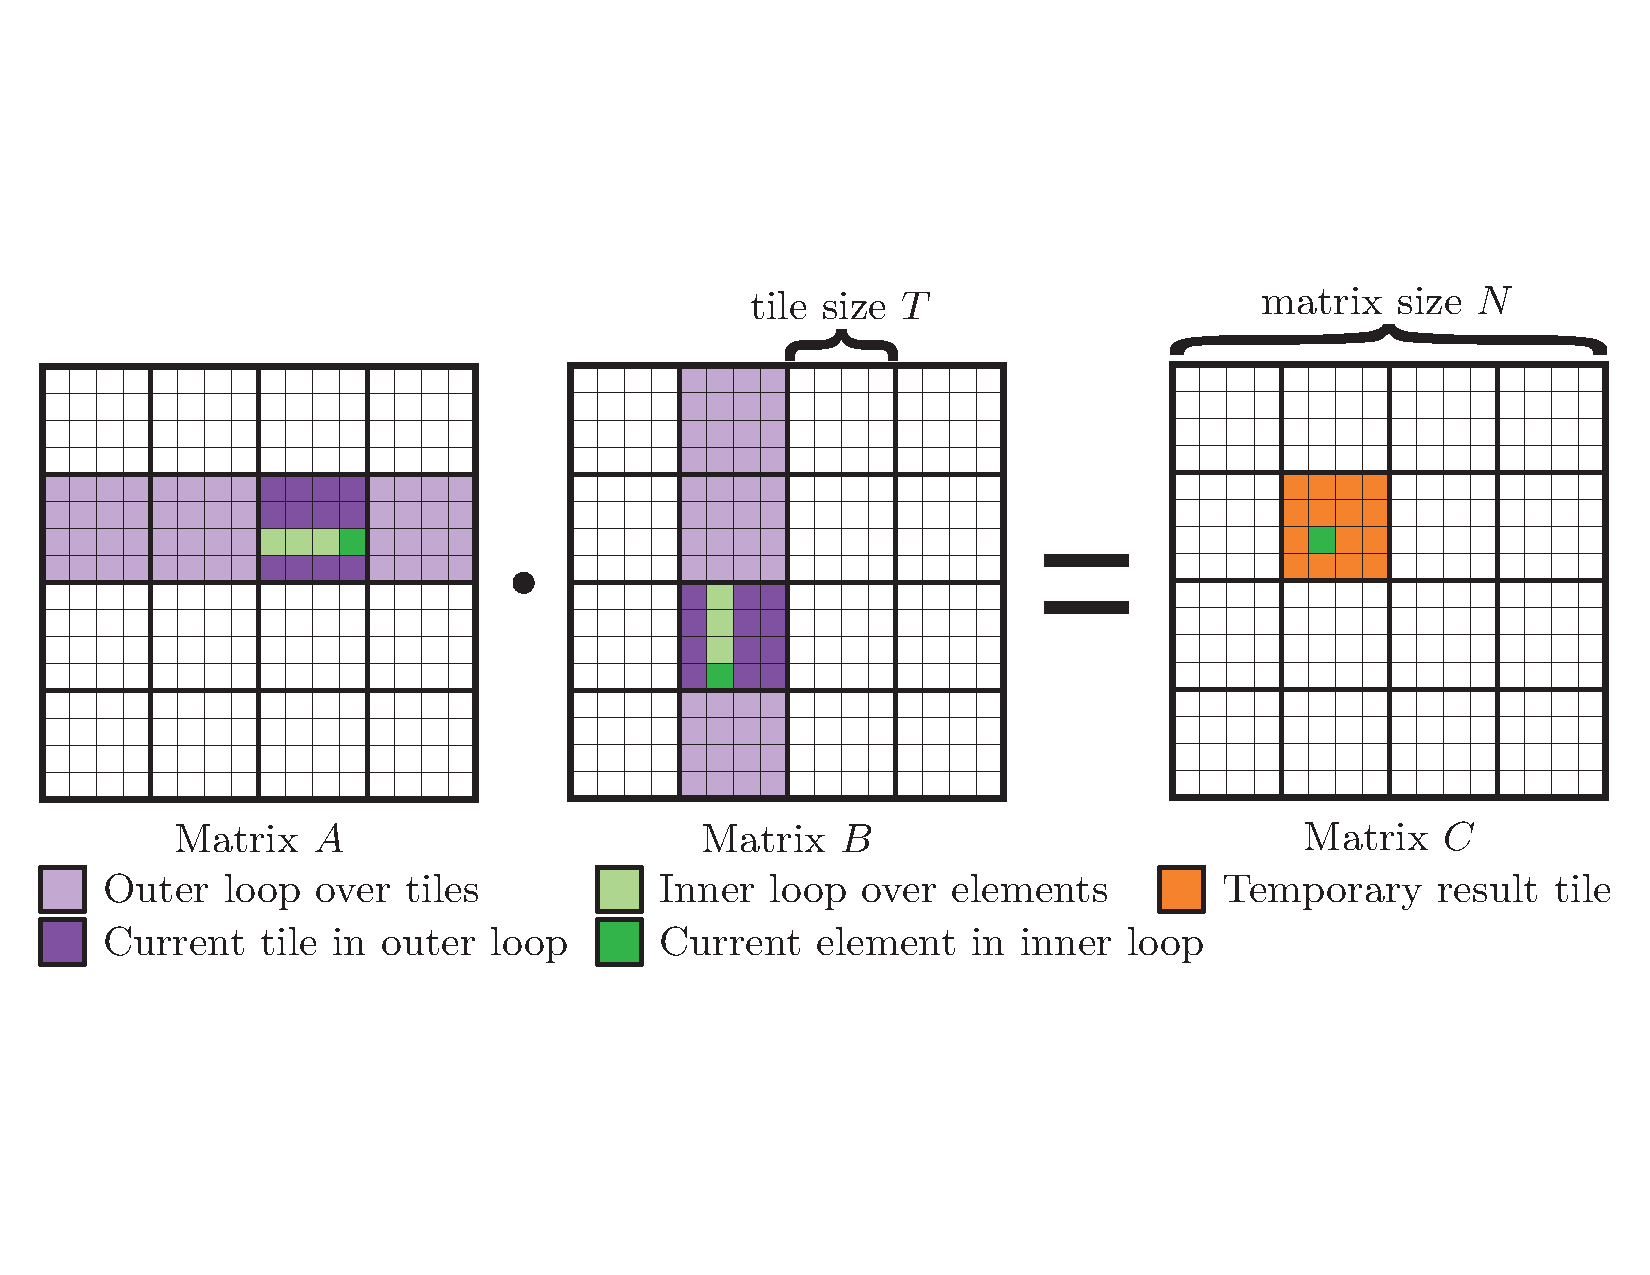
\includegraphics[width=3in]{3_GEMM_backgrounds/tiling.pdf}
    \vspace{-0.5in}
    \caption{An Example of Tiling Strategy}
    \label{fig:tiling}
\end{figure}

Original memory access patterns need to be transformed to adapt to the cache policy of a particular hardware. It is not straightforward to decide an optimal tiling strategy because it requires accurate estimate of accessed array regions in loops to match with cache size of target hardware and meet other constraints. Optimal tiling chooses a tile size for each loop to collectively achieve lowest running time on target hardware.
\subsection{Problem Formulation}
We use TVM~\cite{Chen18} to investigate the performance of matrix tiling for GEMM. TVM facilitates tiling optimization by generating Intermediate Representation (IR) of a particular configuration. Fig.~\ref{fig:gemm_ir} is a simple example IR of GEMM tiling configuration with a blocking factor of 32 on x86 CPU for GEMM with $(m=1024, k=1024, n=1024)$ (short as $(1024,1024,1024)$).
\begin{figure}[htb]
    \centering
    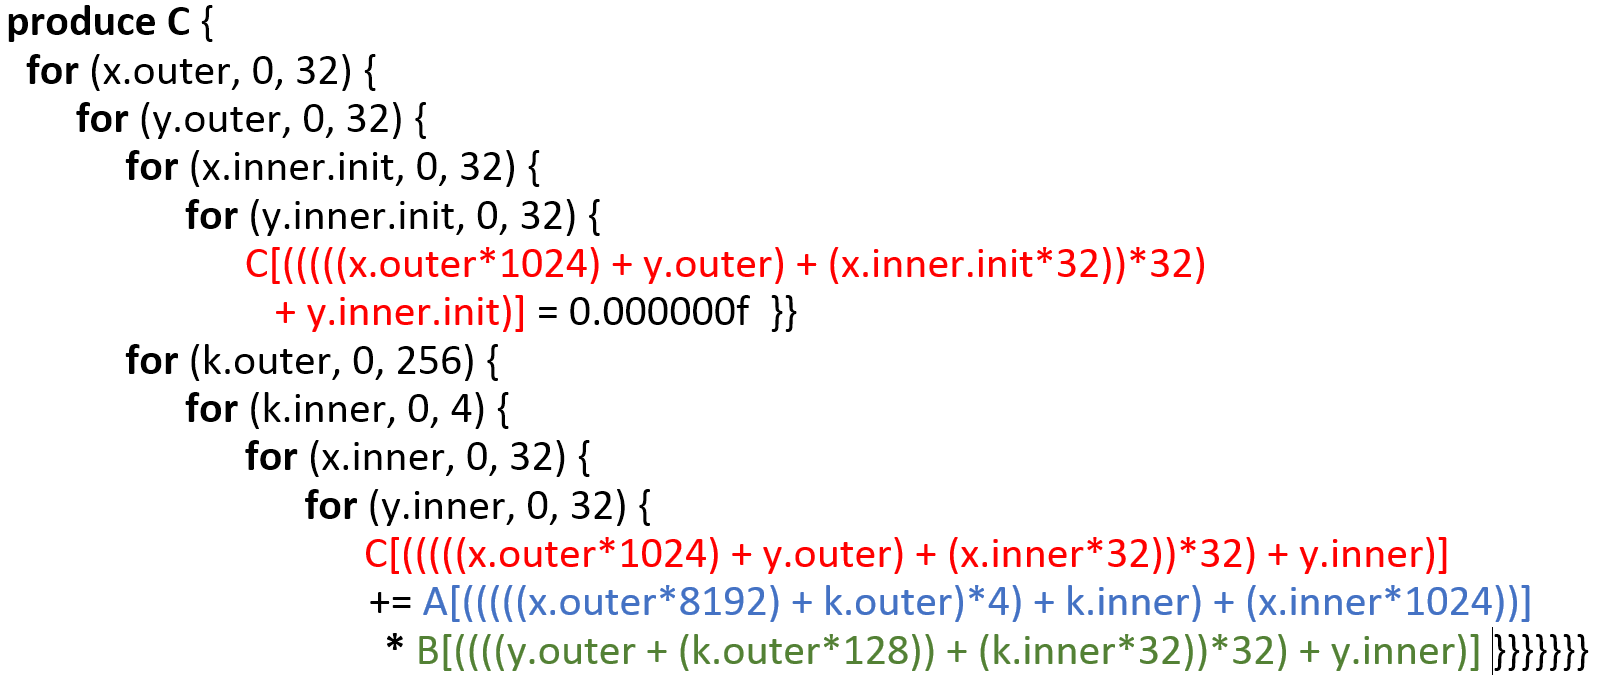
\includegraphics[width=3in]{3_GEMM_backgrounds/gemm_ir.png}
    \caption{IR of GEMM with a blocking factor of 32}
    \label{fig:gemm_ir}
\end{figure}

% \begin{definition}
\noindent
\textbf{Definition:}
Generally, a GEMM tiling configuration can be defined as 
\begin{equation}
    \overrightarrow{\xi} = \overrightarrow{\xi_m} \times \overrightarrow{\xi_k} \times \overrightarrow{\xi_n},
\end{equation}
where
\begin{equation}
     \overrightarrow{\xi_m} =\{ \left[m_0,\ldots,m_i, \ldots m_{d_m-1} \right] |  \Pi_{i=0}^{d_m-1} m_i=m \},
\end{equation}
\begin{equation}
     \overrightarrow{\xi_k} =\{ \left[k_0,\ldots,k_l, \ldots k_{d_k-1} \right] |  \Pi_{l=0}^{d_k-1} k_l=k \},
\end{equation}
\begin{equation}
     \overrightarrow{\xi_n} =\{ \left[n_0,\ldots,n_j, \ldots n_{d_n-1} \right] |  \Pi_{j=0}^{d_n-1} n_j=n \}.
\end{equation}
% \end{definition}
Multiplication of two matrices $A(m\times k)$ and $B(k\times n)$ produces matrix $C(m\times n)$. $d_m$, $d_k$ and $d_n$ are the number of nested loops for each dimension $m$, $k$ and $n$, respectively.  $m_i, k_l, n_j$, $\forall i \in [0, d_m)$ $\forall l \in [0, d_k)$ $\forall j \in [0, d_n)$, are the number of iterations of a respective loop. The configuration in Fig.~\ref{fig:gemm_ir} is $m_0=m_1=32$, $k_0=256, k_1=4$, $n_0=n_1=32$, and $d_m=d_k=d_n=2$.

Constrained by the definition of tiling configuration, we can formulate the following optimization problem:
\begin{equation}\nonumber
    \begin{array}{l}
       \mathop {\min }\limits_{s} T_{cost}(s ; m,k,n,d_m,d_k,d_n).
    \end{array}
\end{equation}
The objective function of this problem is to find an optimal tiling configuration that has minimal running time on target hardware. $T_{cost}$ denotes the running time for the configuration $s$, given the dimension of matrices as $m,k,n$ and the number of the nested loops on each dimension as $d_m, d_k, d_n$. 

%In our experiments, we run GEMM tiling configurations on Nivida CUDA GPU, more specifically $d_m=4$, $d_k=2$ and $d_n=4$.

\section{Methodology}
\subsection{The XGBoost Tuner}

In TVM framework, \cite{Tianqi2018} proposed a configuration tuning method for operator-level optimization in which the search is guided by a performance prediction model trained with eXtreme Gradient Boosting (XGBoost). This XGBoost guided tuner (or XGBoost tuner) follows an iterative search process. In each iteration, a large number of configuration candidates are derived from configuration space by random walk. According to the predicted performance from a trained XGBoost model, the best candidates are selected and tested on hardware. The performance feedback from the hardware is collected and applied to further train the XGBoost model so as to improve its prediction accuracy.

The XGBoost tuner outperforms the other classic tuners including genetic algorithm search, random search, etc., for GEMM. Nevertheless, training the XGBoost model for a large configuration space would incur a high cost. In order to further improve the operator-level configuration tuning performance, we propose a new configuration search model which allows exploitation of relations between similar configurations, followed by two efficient tuning methods.


\subsection{Configuration Search Modeling}

For better analysis, we model the configuration tuning problem as a Markov Decision Process (MDP), where each configuration can be regarded as a unique state. We define the state as follows.

\begin{equation}
    s = \left[ s_m, s_k, s_n, J \right],
\end{equation}
where $s_m = \left[ m_0, m_1, \ldots, m_{d_m-1} \right] \in \xi_m$, $s_k = \left[ k_0, k_1, \ldots, k_{d_k-1} \right] \in \xi_k$, $s_n = \left[ n_0, n_1, \ldots, n_{d_n-1} \right] \in \xi_n$, and $J$ is the binary number indicating whether the state is legitimate (e.g. the product of $m_i$'s must be $m$, the numbers must be integers, etc.).

As in the GEMM application, with similar configuration settings, i.e., the configuration parameters for each dimension of two states are equal or close, the performance of this two states may not exists large difference. Taking advantage of the relations among similar configurations, and considering the constraints of the matrices size in each configuration. We define the concept of action space as follows.

\begin{equation}
    \mathcal{A} = \left[ \begin{array}{l}
         {s_x[i] = 2s_x[i] ~~\text{and}~~ s_x[j]=s_x[j]/2 }, \\ \\
         {\text{where}~ \forall x \in \{m,k,n\}, \forall i, j \in [0, d_x)~\text{and}~ i \neq j }
    \end{array}
     \right].
\end{equation}
Accordingly, we define a step function $step$, i.e.,
\begin{equation}\label{fun:stepfun}
    s'= step(s,a).
\end{equation}
With the input of any action $a \in \mathcal{A}$, the current state $s$ is transferred to state $s'$. We define $s$ and $s'$ are neighbor states. Based on the setting of action space, we guarantee the Euclidean distance between the neighbor state $s$ and $s'$ is the minimum value compared with the distance between the state $s$ and all the other states.

Moreover, in order to better evaluate the performance of each action based on different states, if the agent takes action $a$ and goes from the state $s$ to the state $s'$, we define the rewards as follows
\begin{equation}
    r(s,a) = \frac{1}{T_{cost}(s'; m,k,n,d_m,d_k,d_n) }.
\end{equation}

Following the above modeling, the agent is expected to determine its policy $\boldsymbol{\pi}$ so as to efficiently approach and discover the state $s^*$ with the lowest running time in hardware system. In the following subsections, we will analyze two different configuration tuning approaches guided by G-BFS and N-A2C reinforcement learning, followed by a discussion for their strengths with different scenarios.



\subsection{G-BFS Method}

\begin{figure*}
\centering
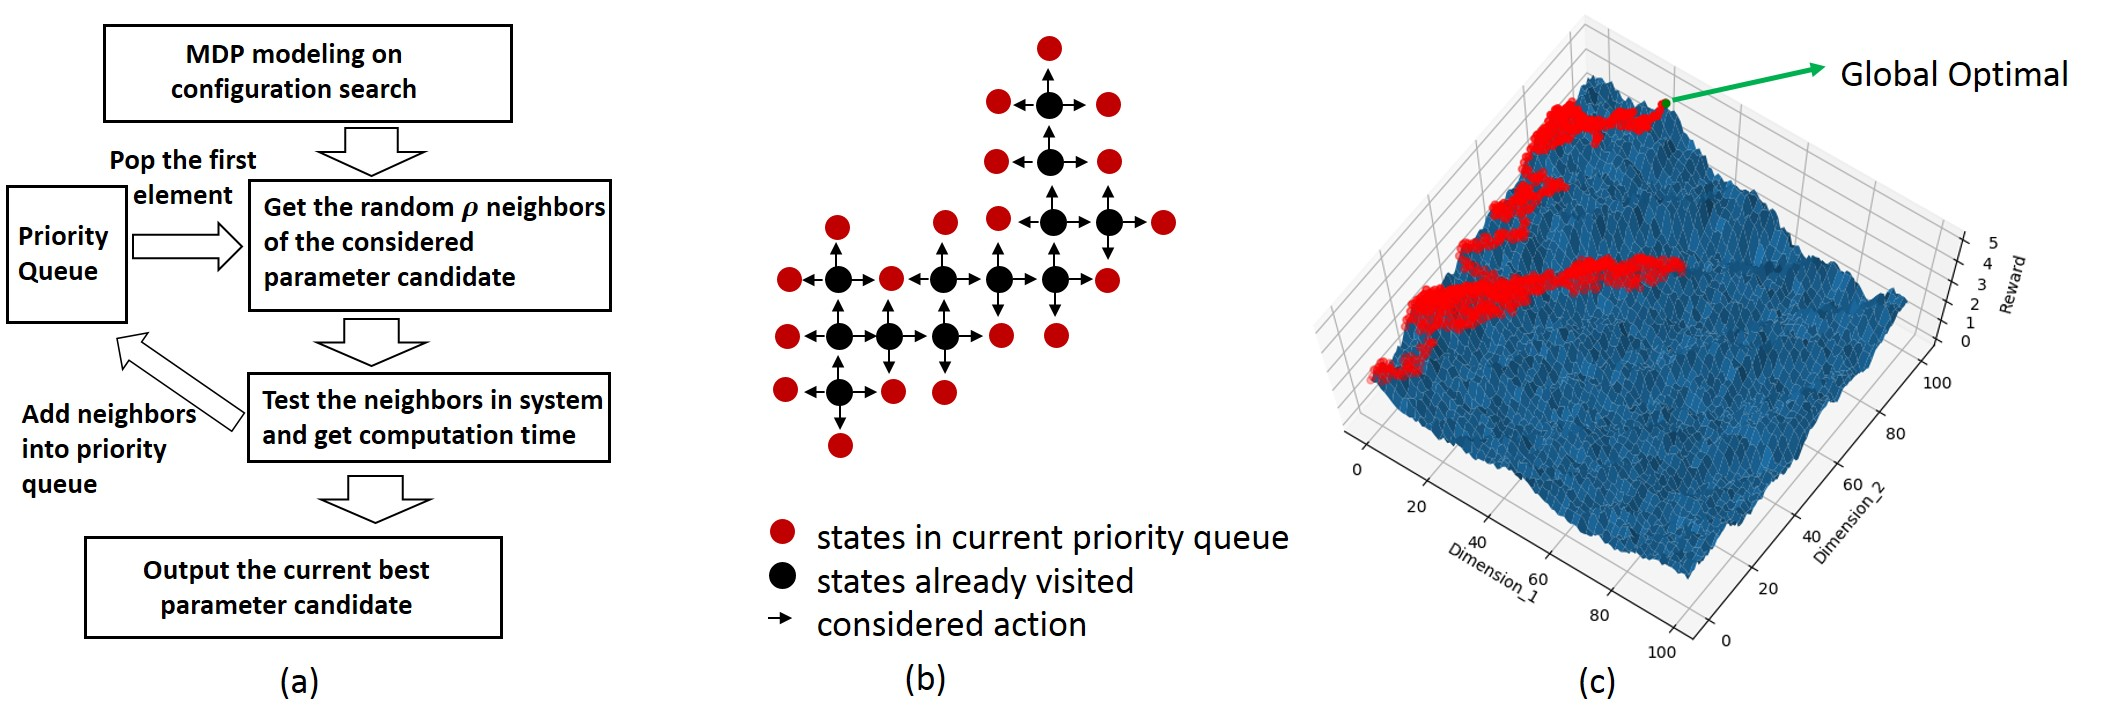
\includegraphics[scale=0.4]{4_Method/gbfs_pic.jpg}
\caption{G-BFS Method}
\label{fig:gbfs}
\end{figure*}

The G-BFS method is guided by Greedy Best-First-Search and follows the flowchart in Fig. \ref{fig:gbfs}(a). We initialize an empty priority queue $\mathcal{Q}$ (ordered by increasing cost), an empty list $S_v$ to record all visited configuration candidates, and a random or hand-crafted starting state $s_0$. We first test and enque the starting state $s_0$ and record its running time $T_{cost}(s_0)$ into the priority queue $Q$. Based on the configuration search model, for each iteration, we deque the top configuration candidate $s$ from the priority queue $Q$. We iterate through all actions $a\in \mathcal{A}$ and collect all corresponding neighbor states as
\begin{equation}
    g(s) = [s'=step(s,a) ~~ \forall a \in \mathcal{A}].
\end{equation}
We randomly select $\rho$ ($\rho \in \{1,2,\ldots,len(g(s)) \}$) configuration candidates from $g(s)$, and test them in hardware. For each state $s'$ sampled from $g(s)$, if state $s'$ is legitimate and has not been visited before, we enque state $s'$ and its tested running time $T_{cost}(s')$ into $Q$ and add state $s'$ in the visited list $S_v$. If its tested running time $T_{cost}(s')$ is smaller than the current minimum running time, we set state $s'$ as the optimal state visited and record its running time as $t_{cost}^{min}$. The iteration continues until the priority queue is empty or the computation time reaches the maximum time specified by the user. The current stored optimal state $s*$ and its running time $t_{cost}^{min}$ are returned as tuning results. The summary of the algorithm is shown in Algorithm \ref{alg:gbfs}.

In Fig. \ref{fig:gbfs}(b), we show the exploration situation in the middle of the tuning algorithm when $\rho = len(g(s))$, where the red nodes denote the state currently stored in the priority queue and the grey nodes are all the visited states. In future iterations, the method will explore from the current most promising red nodes expands its visited state areas. In Fig. \ref{fig:gbfs}(c), we take an example of 2-dimensional configuration search on the randomly generated rewards function. We discover that the proposed G-BFS method is able to correct itself from exploring wrong directions and efficiently expand its neighborhood to the optimal states. Moreover, when the value of $\rho = len(g(s))$, given unlimited tuning time, the algorithm is guaranteed to visit all the configuration states.

\begin{algorithm}[htb]
\caption{G-BFS Method}
\label{alg:gbfs}
\vspace{.1cm}
\hrule
    \begin{algorithmic}[1]
    \vspace{.2cm}
    \STATE Initialization: $\mathcal{Q}$=PriorityQueue(), $S_v$, $s_0$
    \STATE Q.push($(T_{cost}(s_0), s_0)$);\\
    \STATE Add $s_0$ in $S_v$;\\
    \WHILE{$Q\neq \O$ and $t<T^{max}$}
        \STATE $(T_{cost}(s), s)$ = Q.pop(); \\
        \STATE $\mathcal{B}_{test}$ = Sample $\rho$ randomly from $g(s)$; \\
        \FOR{$s'$ in sampled configuration candidates}
            \IF{$s'[-1]=True$ and $s' \not\in S_v$}
                \STATE Q.push($(T_{cost}(s'), s')$); \\
                \STATE Add $s'$ in $S_v$;\\
                \IF{$t_{cost}^{min} > T_{cost}(s')$}
                    \STATE $t_{cost}^{min} = T_{cost}(s')$; \\
                    \STATE $s^* = s'$;
                \ENDIF
            \ENDIF
        \ENDFOR
    \ENDWHILE
    \STATE Return: The optimal configuration $s^*$ with cost $t_{cost}^{min}$.
    \end{algorithmic}
\hrule
\end{algorithm}






\subsection{N-A2C Method}






\begin{algorithm}[htb]
\caption{N-A2C Method}
\label{alg:r_a2c}
\vspace{.01cm}
\hrule
    \begin{algorithmic}[1]
    \vspace{.2cm}
    \STATE Initialization: {$s_0$, $\mathcal{M}$, $H_v$}
    \FOR{each episode}
        \WHILE{$len(\mathcal{B}_{collect})< len(\mathcal{B}_{test})$ }
            \STATE$s = s_0$; \\
            \FOR{each step until $T$ steps}
                \IF{$rand()<\tau$}
                    \STATE $a$ follows $\pi(s)$;
                \ELSE
                    \STATE $a$ is random selected from $\mathcal{A}$;
                \ENDIF
                \STATE $s'=step(s,a)$; \\
                \IF {$s'$ not in $H_v$}
                    \STATE Add $s'$ in $\mathcal{B}_{collect}$;
                \ENDIF
                \STATE $s = s'$;
            \ENDFOR
        \ENDWHILE
        \FOR{$s'$ in $\mathcal{B}_{collect}$}   % Can be done in parallel computing
            \IF{$t_{cost}^{min} > T_{cost}(s')$}
                \STATE $t_{cost}^{min} = T_{cost}(s')$; \\
                \STATE $s^* = s'$; \\
                \STATE $s_0=s^*$; \\
            \ENDIF
            \STATE $H_v[s'] = T_{cost}(s')$; \\
            \STATE Store $(s, a, r(s,a), s')$ to $\mathcal{M}$, where $\forall s$, $\forall a$ satisfying $step(s,a) = s'$; \\
            \STATE Train actor's and critic's neural networks with $\mathcal{M}$;
        \ENDFOR
    \ENDFOR
    \STATE Return: The optimal configuration $s^*$ with cost $t_{cost}^{min}$.
    \end{algorithmic}
    \hrule
\end{algorithm}

As the G-BFS method explores only one step from the considered state for each iteration, its performance may be affected when the running time from similar states exhibits large random noise. In the N-A2C method, as shown in Fig. \ref{fig:r_a2c}(a), for each episode, we let the exploration being generated in a $\varsigma$-step neighborhood, and the direction of exploration is guided with A2C reinforcement learning method \cite{bhatnagar2009natural}. The center of the exploration neighborhood is periodically updated with the optimal states ever visited.


We summarize the tuning method in Algorithm~\ref{alg:r_a2c}. Initially, we set a random or experience-estimated starting state $s_0$, a fixed-size memory buffer $\mathcal{M}$ to record the latest searching information and an empty hashtable $H_v$ recording all the visited states with their running time. For the A2C reinforcement learning model, both actor and critic firstly establish their neural networks with random weights, respectively. Following the configuration search model, for each episode, while the collected configuration candidates for testing is less than the predefined tested batch size, iteratively, from the same starting point, the agent explore $\mathcal{T}$ continuous steps. For each step, with probability of $\tau$, the agent take action $a$ guided by the policy $\pi(s)$ from the actor's nerual network; With probability of $1-\tau$, the agent choose a random action $a$ from current state. Based on the current state $s$ and action $a$, we get the next state $s'$ from (\ref{fun:stepfun}). If the next state $s'$ has not been visited before, we add the state $s'$ in collected candidate batch $\mathcal{B}_{collect}$.




When the number of collected candidates $\mathcal{B}_{collect}$ achieve the predefined test size, we let the system run the collected configuration candidates. Based on the corresponding running time, the stored hashmap $H_v$ and memory buffer $\mathcal{M}$ is updated. Based on updated $\mathcal{M}$, by randomly selecting history exploration data, the neural networks of A2C reinforcement learning is trained.



Generally, the proposed N-A2C method is able to efficiently search the optimal GEMM configuration with fixed exploration step in each episode. Nevertheless, in order to find the most important exploration neighborhood, the exploration step $\mathcal{T}$ can have a soft start, which means starting with a large value and gradually reduce to a small number. Moreover, in order to fully explore the configuration space, after a long time exploration within the same starting points, the exploration step $\mathcal{T}$ will gradually increase to further explore new configuration candidates.

In Fig. \ref{fig:r_a2c}(b), we show a simple exploration map with the proposed N-A2C method. With more explorations, the exploration neighborhood changes with the update of optimal states ever visited. In Fig. \ref{fig:r_a2c}(c), we take an example of 2-dimensional configuration on the randomly generated rewards function. Due to the large randomness in the example, we set the exploration step $\mathcal{T}$ as 100 and the global optimal state can be efficiently discovered with the assistance of the A2C reinforcement learning algorithm.

\begin{figure*}
\centering
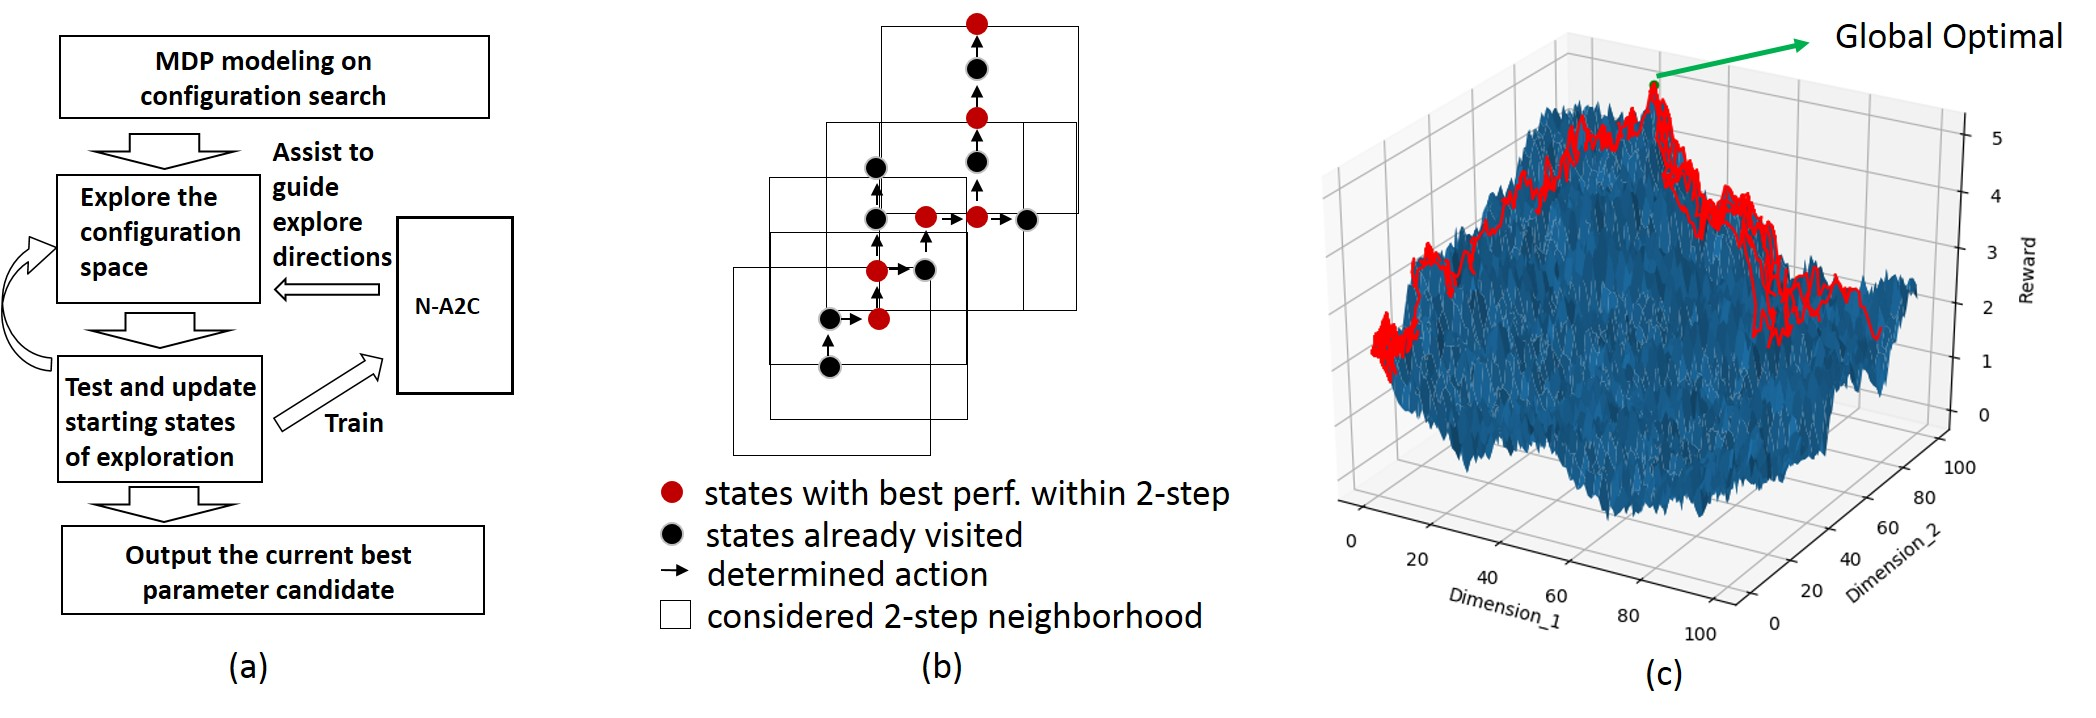
\includegraphics[scale=0.4]{4_Method/n_a2c_pic.jpg}
\caption{N-A2C Method}
\label{fig:r_a2c}
\end{figure*}


\subsection{Discussion}
We compare the G-BFS guided tuning method, N-A2C reinforcement learning method and the XGBoost guided tuning method in Table \ref{tab:compare}.

\begin{table}[h!]
    \small
    \begin{center}
        \caption{Comparison of Configuration Search Methods}
        \label{tab:compare}
        \begin{tabular}{l|c|c|c}
            Methods & XGBoost  & G-BFS & N-A2C \\
            \hline
 %           Explore neighbor conf. & No & Yes  & Yes  \\
            Adapt to large space & No & Yes & Yes \\
            Adapt to fluctuations & Weak & Weak & Strong \\
 %           Random Exploration & Exist & Depend & Exist \\
            Lightweight & No & Yes & Yes \\
            Hyper-parameters & Yes & only 1 & Yes \\
            Trapped in Local Optima & No & No & No
        \end{tabular}
    \end{center}
\end{table}

Since our proposed configuration search model is based on neighborhood information which is the ground for both our tuners, exploration by G-BFS and N-A2C methods are more confined in neighborhoods of current candidates and increasing the size of the configuration space does not have a large impact as it does on the XGBoost method, as the XGBoost method considers the overall configuration space.  Furthermore, when the performance feedback of neighboring configurations has large fluctuations, XGBoost and G-BFS may not be able to efficiently discover the global optimal solution, while the N-A2C method can explore multiple steps from the neighborhood, so as to locate the optimal configuration more efficiently. Moreover, random exploration exists within both XGBoost and N-A2C tuning methods, but in G-BFS, when the value of $\rho = len(g(s))$, there will be no randomness during the configuration search. Compared with other configuration optimization methods, G-BFS is more lightweight and only requires the hyper-parameter setting of $\rho$. Finally, all three methods are able to jump out of  local optima to get to global optimal solutions.



\section{Experimental Results}
\begin{figure}[t]
    \centering
    \begin{subfigure}[b]{0.45\textwidth}
    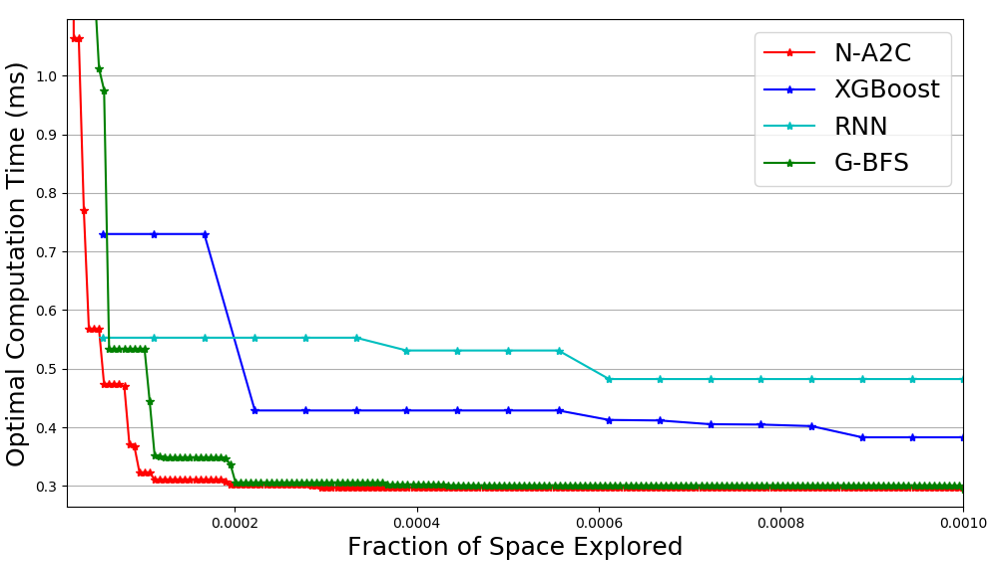
\includegraphics[width=\linewidth]{5_Simu/simu_11.png}
    \caption{Optimal computation time versus ratio of visited data}
    \label{fig:simu11}
    \end{subfigure}
    \hspace{0.2in}
    \begin{subfigure}[b]{0.45\textwidth}
    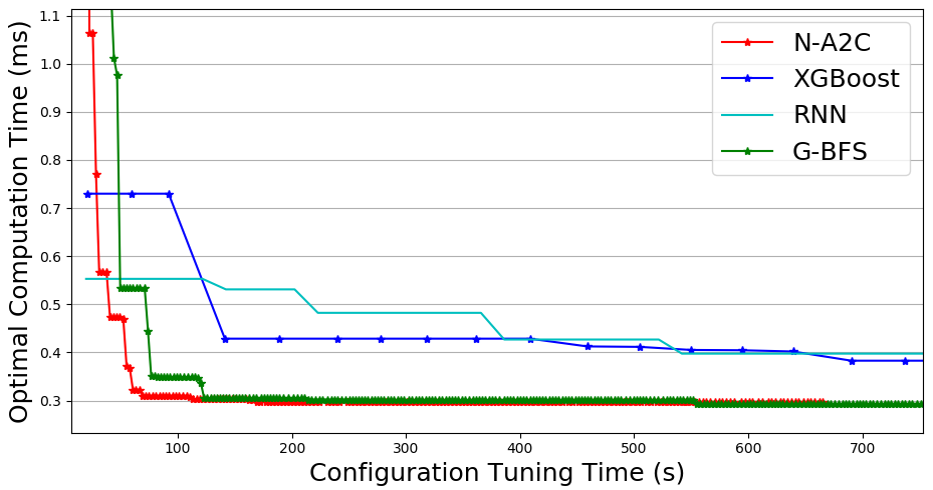
\includegraphics[width=\linewidth]{5_Simu/simu_12.png}
    \caption{Optimal computation time versus searching time}
    \label{fig:simu12}
    \end{subfigure}
    \caption{GEMM configuration tuning in (1024, 1024, 1024)}
    \label{fig:1024}
\end{figure}




Performance of the proposed GEMM configuration tuning approaches is evaluated in the TVM framework on Nvidia Titan Xp GPU. Following similar settings in TVM for GPUs, we set the number of nested loops for each dimension as $d_m=4, d_k=2, d_n=4$. We set the random selection parameter $\rho=5$ for the G-BFS method, and the maximum search step $\mathcal{T} =3$ for the N-A2C method. For generality, we set the initial state for the proposed methods as $s_0 = [[m,1,1,1],[k,1],[n,1,1,1]]$, referring to the situation without multi-level matrix tiling, and the performance of our proposed methods can be further improved by setting the initial state to a more meaningful configuration. In order to investigate the performance of our proposed methods, we compare them with the state-of-the-art algorithms including the XGBoost guided configuration tuning methods (or "the XGBoost method") in TVM framework and the general configuration optimization method using a RNN controller by Google researchers. Without specific explanations, the computation time for each configuration is the arithmetic mean for 10 repeated trials on the tested GPU hardware.

In simulations, we evaluate and compare the configuration tuning efficiency in a perceptron network, which is the fundamental unit for state-of-the-art neural network architectures and mainly includes GEMM for computation. During training of the network, we denote the setting of neural network in the format of $(number_of_inputs,batch_size,number_of_outputs)$, which corresponds to $(m,k,n)$ in matrices $A(m \times k)$ and $B(k \times n)$ for GEMM.

% In Fig. \ref{fig:1024}, we set the size of matrices $A(m \times k)$ and $B(k \times n)$ as $m=1024, k=1024, n=1024$

In Fig. \ref{fig:1024}, we set $number_of_inputs=1024$, $batch_size=1024$ and $number_of_outputs=1024$, and show the performance of our proposed configuration tuners. We first analyze the optimal computation time discovered with respect to the fraction of visited configurations in Fig. \ref{fig:simu11}. Based on the sizes of matrices and the number of nested loops, there are totally $899756$ configuration candidates. With the value of visited fraction increasing, the optimal computation time discovered generally decreases. Compared with the XGBoost and RNN methods, the proposed N-A2C and G-BFS methods are able to discover the configuration candidate with lower fraction of visited configuration candidates. Fig. \ref{fig:simu12} plots the optimal cost (hardware computation time) discovered by the four methods as tuning progresses over time. The proposed N-A2C and G-BFS methods generally use less tuning time to find the configuration with lower cost, compared with the XGBoost and RNN methods.

\begin{figure}[t]
    \centering
    \begin{subfigure}[b]{0.42\textwidth}
    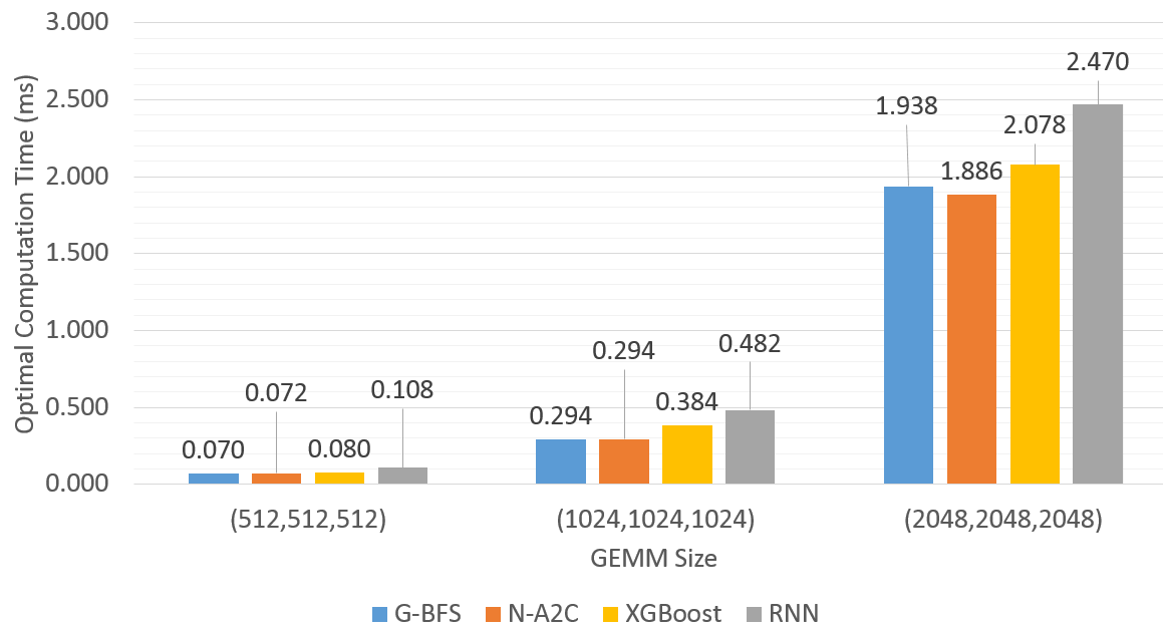
\includegraphics[width=\linewidth]{5_Simu/simu_21.png}
    \caption{When the fraction of visited configurations reaches 0.1\%}
    \label{fig:simu21}
    \end{subfigure}
    \hspace{0.2in}
    \begin{subfigure}[b]{0.42\textwidth}
    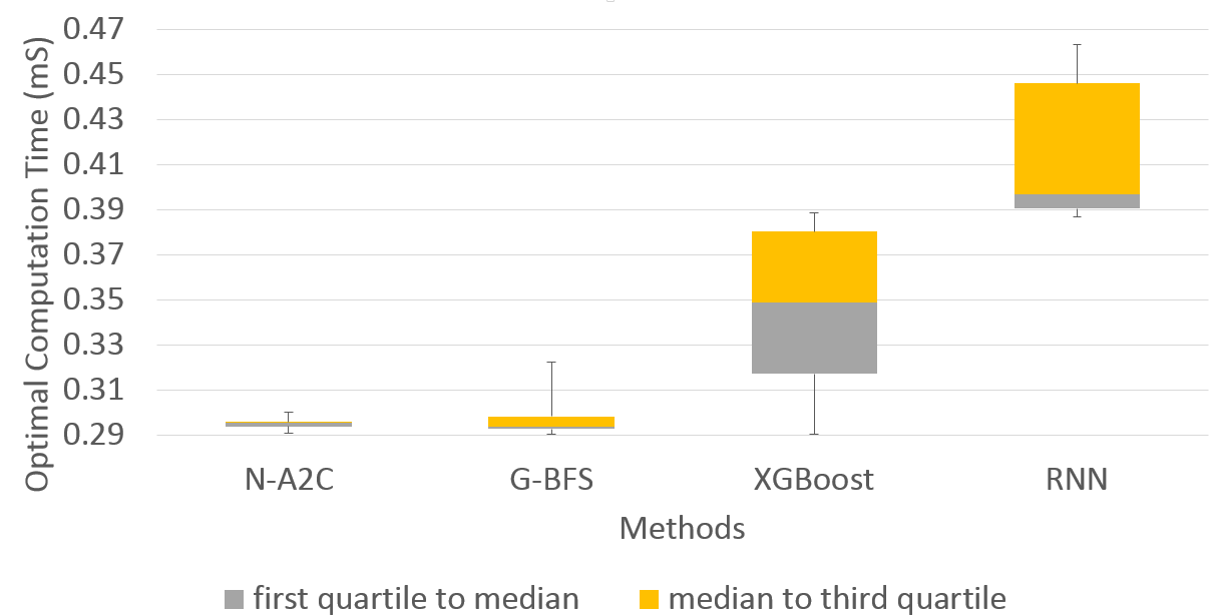
\includegraphics[width=\linewidth]{5_Simu/simu_23.png}
    \caption{When the tuning time reaches 750 seconds}
    \label{fig:simu23}
    \end{subfigure}
    \caption{Comparisons of configuration tuning efficiency}
    \label{fig:multi_case}
\end{figure}


In Fig. \ref{fig:multi_case}, we evaluate and compare the configuration tuning efficiency in the perceptron network. In Fig. \ref{fig:simu21}, we compare the discovered optimal computation time when the fraction of visited configuration candidates reaches 0.1\%. The total numbers of configuration candidates for $(512, 512, 512)$, $(1024, 1024, 1024)$, $(2048, 2048, 2048)$ matrix tiling are $484000$, $899756$ and $1589952$, respectively. As the sizes of matrices increase, longer computation time is required, and G-BFS and N-A2C can search configuration more efficiently than the XGBoost and RNN methods. Specifically, with 0.1\% exploration of $(1024, 1024, 1024)$'s configuration space, the proposed G-BFS and N-A2C methods are able to discover configurations of 24\% lower computation time than what the XGBoost method can find and configurations of 40\% lower computation time than what the RNN method can find. When the sizes of matrices increase, the N-A2C method outperform G-BFS method, as the N-A2C method is able to go multiple steps from the current state. In Fig. \ref{fig:simu23}, we compare the optimal discovered computation time of a configuration when the tuning time is limited to 750 seconds. In order to show the variance of performance incurred by random exploration for each method, we draw a box plot with the minimum, first quartile, median, mean, third quartile, and maximum values during the 10 trials on the $(1024, 1024, 1024)$ tiling. We can see that our methods exhibit more stable performances than the other two methods.


%However, due to the configuration optimization, the computation time for large matrices is much faster than the addition of the computation time of multiple small matrices divided from the large matrices.




\section{Conclusion}
In this paper, we propose a Greedy Best First Search guided (G-BFS) method and a Neighborhood Actor Advantage Critic (N-A2C) method for compiler-level GEMM optimization, taking advantage of performance of neighborhood configurations. The G-BFS method, though being lightweight, have shown strength of stable performance; and the N-A2C method performs better for large matrices. Empirical results show that both methods achieve significant performance improvement over  state-of-the-art tuning methods such as those using XGBoost and RNN controller. Both methods are general in the sense that they are applicable to other compiler-level tuning tasks and can be used for optimization of other tensor operators with large configuration space.

{
\begin{spacing}{0.92}
\footnotesize
\bibliographystyle{icml2019}
\bibliography{icml}
\end{spacing}
}

\end{document}
